\documentclass[article]{jss}

%% -- LaTeX packages and custom commands ---------------------------------------

%% recommended packages
\usepackage{orcidlink,thumbpdf,lmodern}

\usepackage[american]{babel}
\usepackage{amsmath}
\usepackage{amssymb}%
\usepackage{mathrsfs}
\usepackage{amsbsy}
\usepackage{amsthm}
\usepackage{float}
\usepackage{amsmath}
\usepackage{booktabs}

%% new custom commands
\newcommand{\class}[1]{`\code{#1}'}
\newcommand{\fct}[1]{\code{#1()}}

%% For Sweave-based articles about R packages:
%%\SweaveOpts{engine = R, eps = FALSE, pdf = TRUE, keep.source = TRUE, prefix.string = spca_JSS}


%% -- Article metainformation (author, title, ...) -----------------------------

%% - \author{} with primary affiliation (and optionally ORCID link)
%% - \Plainauthor{} without affiliations
%% - Separate authors by \And or \AND (in \author) or by comma (in \Plainauthor).
%% - \AND starts a new line, \And does not.
\author{Giovanni Maria Merola~\orcidlink{0000-0003-2539-9225}\\
British University Vietnam}
\Plainauthor{Giovanni Maria Merola} 

%% - \title{} in title case
%% - \Plaintitle{} without LaTeX markup (if any)
%% - \Shorttitle{} with LaTeX markup (if any), used as running title
\title{An R package to Compute Least Squares Sparse Principal Components}
\Plaintitle{An R package to compute Least Squares Sparse Principal Components}
\Shorttitle{An \proglang{R} package to compute LS-SPCA components}

%% - \Abstract{} almost as usual
\Abstract{
This article illustrates the use of the package \emph{spca}. The computation of sparse principal components is carried out with the LS-SPCA approach. This approach is different from all othe SPCA method because it is based on data approximation, rather than components with largest variance. The article  includes  a brief introduction to LS-SPCA theory and an extended SPC analysis of a small dataset. Most of the options are mentioned and used. Further details can be found in the package documentation.}

%% - \Keywords{} with LaTeX markup, at least one required
%% - \Plainkeywords{} without LaTeX markup (if necessary)
%% - Should be comma-separated and in sentence case.
\Keywords{JSS, style guide, comma-separated, not capitalized, \proglang{R}}
\Plainkeywords{JSS, style guide, comma-separated, not capitalized, R}
\Keywords{JSS, SPCA, Least squares, projection, uncorrelated, \proglang{R}}
\Plainkeywords{JSS, SPCA, Least squares, projection, uncorrelated, R}


\Address{
  Giovanni Merola\\
  British University Vietnam\\
  Ecopark, Hung Yen\\
  Vietnam\\
  E-mail: \email{merolagio@gmail.com}\\
}

% to use latex macros inside r chunks
% <<results='asis'>>=
% cat("\\[ \\bX = \\bA \\trans \\]\n")



%% \codo allows to use of underscores ========================
\makeatletter
\newcommand\codo{%
  \begingroup
  \@makeother\_\@makeother\~\@makeother\$\@codox
}
\def\@codox#1{%
  {\normalfont\ttfamily\hyphenchar\font=-1 \detokenize{#1}}%
  \endgroup
}
\makeatother


%%%%%%%%%%%%%%%%%%%%%%%%%%%%%%%%%%%%%%%%%%%%%%%%%%%%%%%%%%%%%%%%%%%%%%%%%%%%%%%%%%%%%%
\newcommand{\trasp}{^{\scriptstyle{\intercal}}}
\newcommand{\traspj}{^{\scriptstyle{\intercal}}_j}
\newcommand{\trasps}[1]{^{\raisebox{\depth}{$\scriptstyle{\intercal}$}}_{#1}} %use without overset symbol
\newcommand{\traspd}[1]{^{\raisebox{-1.0mm}{$\scriptstyle{\intercal}$}}_{#1}} %use with overset symbol
\newcommand{\traspdb}[1]{^{\raisebox{-1.0mm}{$\scriptstyle{\intercal}$}}_{[#1]}}
%use with overset symbol and subscript in []
\newcommand{\traspdr}[1]{^{\raisebox{-1.0mm}{$\scriptstyle{\intercal}$}}_{(#1)}}
%use with overset symbol and subscript in ()

\newcommand{\Xj}{{{X}_j}}
\newcommand{\XjT}{{{X}\trasps{j}}}
\newcommand{\Qj}{{{Q}_j}}
\newcommand{\QjT}{{{Q}\trasps{j}}}
 \newcommand{\bQj}{{\mathbf{Q}_j}}
\newcommand{\bQjT}{{\mathbf{Q}\trasps{j}}}
 \newcommand{\bQ}{{\mathbf{Q}}}
\newcommand{\bXj}{{\mathbf{X}_j}}
\newcommand{\bXjT}{{\mathbf{X}\trasps{j}}}
\newcommand{\bX}{{\mathbf{X}}}
\newcommand{\dajT}{{\overset{\boldsymbol{.}}{a}\traspd{j}}}
\newcommand{\daj}{{\overset{\boldsymbol{.}}{a}_j}}


\newcommand{\dA}{{\overset{\boldsymbol{.}}{A}}}
\newcommand{\dAj}{{\overset{\boldsymbol{.}}{A}_j}}
\newcommand{\dAjT}{{\overset{\boldsymbol{.}}{{A}}\traspd{j}}}
\newcommand{\da}{{\overset{\boldsymbol{.}}{a}}}
% \newcommand{\daj}{{\overset{\boldsymbol{.}}{a}_j}}
% \newcommand{\dajT}{{\overset{\boldsymbol{.}}{{a}}\traspd{j}}}
\newcommand{\dX}{{\overset{\boldsymbol{.}}{X}}}
\newcommand{\dXj}{{\overset{\boldsymbol{.}}{X}_j}}
\newcommand{\dXjT}{{\overset{\boldsymbol{.}}{{X}}\traspd{j}}}
\newcommand{\dQ}{{\overset{\boldsymbol{.}}{Q}}}
\newcommand{\dQj}{{\overset{\boldsymbol{.}}{Q}_j}}
\newcommand{\dQjT}{{\overset{\boldsymbol{.}}{Q}\traspd{j}}}
\newcommand{\dS}{{\overset{\boldsymbol{.}}{S}}}
\newcommand{\dST}{{\overset{\boldsymbol{.}}{S}\trasp}}
\newcommand{\dSj}{{\overset{\boldsymbol{.}}{S}_j}}
\newcommand{\dSjT}{{\overset{\boldsymbol{.}}{S}\traspd{j}}}


\newcommand{\vexp}{\emph{vexp}}
\newcommand{\vexpq}{\emph{vexp}_Q}
\newcommand{\evexp}{\emph{evexp}}


\DeclareMathOperator*{\argmin}{arg\,min}
\DeclareMathOperator*{\argmax}{arg\,max}


%% internal
%% these are for the matrix Q_T_[j-1] -- argument is the matrix T (or Y or Z, etc)
\newcommand{\traspsM}[1]{^{\raisebox{\depth}{$\scriptstyle{\intercal}$}}_{{#1}_{[j - 1]}}} %use without overset symbol
\newcommand{\traspdM}[1]{^{\raisebox{-1.0mm}{$\scriptstyle{\intercal}$}}_{{#1}_{[j - 1]}}} %use with overset symbol and
%\newcommand{\traspdMM}[1]{^{\raisebox{-2.0mm}{$\scriptstyle{\intercal}$}}_{{#1}_{[j - 1]}}} %use with overset symbol and subscript in []
\newcommand{\traspsMb}[1]{^{\raisebox{\depth}{$\scriptstyle{\intercal}$}}_{\mathbf{#1}_{[j - 1]}}} %use without overset symbol
\newcommand{\traspdMb}[1]{^{\raisebox{-1.0mm}{$\scriptstyle{\intercal}$}}_{\mathbf{#1}_{[j - 1]}}} %use with overset symbol and


\newcommand{\matinv}{^{\raisebox{+1.0mm}{$\scriptstyle{{-1}}$}}} %use for matrices
\newcommand{\matinvj}[1]{^{\raisebox{-1.0mm}{$\scriptstyle{{-1}}$}}_{#1}} %use for matrices with overset symbol
\newcommand{\matinvjb}[1]{^{\raisebox{-1.0mm}{$\scriptstyle{{-1}}$}}_{[#1]}} %use for matrices with overset symbol and subscript in []
\newcommand{\matginv}{^{\raisebox{+1.0mm}{$\scriptstyle{{+}}$}}} %use for matrices
%%%%%%%%%%%%%%%%%%%%% Ignoring Font Warnings %%%%%%%%%%%%%%%%%%%%%%%%%%%%%%
%



\usepackage{Sweave}
\begin{document}
%% changed to FALSE

%% changed to FALSE


\section{Introduction}
Principal components analysis (PCA) is a standard method for reducing the dimensionality of multivariate data. PCA replaces the original variables with linear combinations, the principal components (PCs), ordered by decreasing variance explained. The first few PCs often summarize a substantial proportion of the variation in the data. This is obtained by requiring that the PCs best approximate the data in a least-squares (LS) sense.

The PCs are difficult to interpret when the number of variables is large, because all the variables contribute to each component. Furthermore, the popular method of considering only `large' loadings for their interpretation leads to selecting highly correlated variables, which, as an ensemble, have little data approximation power \citep{mer20}. Sparse principal components analysis (SPCA) addresses this problem by computing \emph{sparse} principal components (sPCs) that are linear combinations of only a few of the variables. Hence, several coefficients of these linear combinations, called \emph{loadings}, are zero, which makes the identification of the important variables that define the sPCs easier. 


The first SPCA method was proposed by \cite{tre}; since then, a plethora of other SPCA methods have been proposed. These \emph{conventional} SPCA methods compute by imposing sparsity constraints to the PCA objective of maximizing the variance of sPCs proposed by \citet{hot}. 

Conventional SPCA methods differ because there is no agreement on the sparsity constraints to impose and on how to transform the data after sPCs are computed to avoid computing the same solution. This lack of agreement led to sophisticated optimization approaches for different objective functions that provide competing solutions. Often the resulting sPCs are not close to the original PCs. The review articles in the series \emph{All sparse PCA models are wrong, but some are useful} (\citeauthor{camI}, \citeyear{camI}, \citeyear{camII}, \citeyear{camIII}) analyze many existing conventional SPCA methods. \citet{mer19} also discusses additional drawbacks of these methods.

LS-SPCA was first proposed by \citet{mer15} and its projection variant by \citet{mer19}. This approach computes sPCs that best approximate the data in a least--squares (LS) sense, imposing sparsity directly on Pearson's classic PCA data-approximation objective \citep{pea}. Notably, while Pearson's and Hotelling's objectives give the same solutions in standard PCA, they differ once sparsity constraints are introduced \citep{mer15, mer19}. This helps explain why \citeauthor{camI} concluded that all conventional SPCA methods are wrong.

The difference between LS-SPCA and conventional SPCA is important for applications. LS-SPCA finds genuine sparse approximations to the Pcs. 
Since the inclusion of highly correlated variable in the subset defining the sPCs will not increase the variance explained by much, it is very likely that LS-SPCA identifies subsets of variable with low multiple correlation.
The sPCs computed with conventional SPCA are the leading PCs of subsets of the variables chosen to yield the largest possible first eigenvalue. Hence, the remaining variables are disregarded and the variables selected need to be as highly multiply correlated as possible. 

The \pkg{spca} package efficiently computes LS-SPCA solutions and provides helper functions to visualize and compare them. 
The main computations are carried out by the \proglang{C++} back-end. The architecture is design to save computational effort, for example by using a reverse-SVD approach for `fat` matrices. Three methods are available to print, plot, summarize the results, additionally there are helpers for comparing different fits and computing standard PCA and storing the results as an \class{spca} object. Rather than a black-box optimizer, \pkg{spca} it provides a flexible and intuitive user interface with transparent options and goodness--of--fit metrics.

This article also serves as an extended package vignette. It therefore illustrates the main options and helper functions needed to conduct a complete SPCA analysis. Tables in the illustration section are printed as they appear in an interactive \proglang{R} session. The next section briefly introduces the theory behind LS-SPCA. Section~\ref{sec:spcapack} illustrates the package through examples.

\section{LS-SPCA methodology}\label{sec:spcapack}
The material in this section is taken from \citet{mer15} and \citet{mer19}, where proofs and further details can be found. 

We first establish notation. Let $X$ denote the $n \times p$ data matrix, containing $n$ cases on $p$ features centered to mean zero, and let $S \propto X\trasp X$ denote the covariance matrix. The eigenvectors of $S$, $v_1, \ldots, v_p$ ($\vert\vert v_j \vert\vert = 1$, $j = 1, \ldots, p$), are the PC loadings and are ordered by decreasing corresponding eigenvalues,
$\lambda_1 \geq \lambda_2 \geq \cdots \geq \lambda_p$. The same convention is used for all eigenvectors, including generalized eigenvectors.

The $r \leq p$ sparse loading $p$-vectors are denoted by $a_j$, $j = 1,\ldots,r$, have unit norm $a\traspj a_j = 1$, and each has only $c_j \leq p$ nonzero elements. The quantity $c_j$ is the \emph{cardinality} of $a_j$. The sPC scores, or simply sPCs, are then $t_j = Xa_j$.

A dot above a symbol denotes the operation of retaining the elements of a vector, or the columns of a matrix, corresponding to a set of indices $ind_j$. In \proglang{R} syntax, $\daj = a_j[ind_j]$ is the vector containing only the $c_j$ nonzero loadings in $a_j$, so that $t_j = \dXj\da_j$.

\subsubsection{LS-SPCA objective}
As mentioned, the LS-SPCA objective is obtained by imposing sparsity constraints on the standard PCA least--squares data-approximation objective. This is equivalent to maximizing the variance explained (VEXP) by each PC. The objective can be expressed recursively as
\begin{equation}\label{eq:lsscpca_obj}
\min_{a_j} \|X - t_j b_j\trasp\|^2,
\quad \text{subject to}\quad
\operatorname{card}(a_j) < p,
\quad a\traspj S a_i = 0,\ i < j;\ j = 1, \ldots, r,
\end{equation}
where the vectors $b_j$ are regression coefficients that are not of interest.

Our approach is to separate the computation of the solutions into two steps:
\begin{enumerate}
\item Define how to compute the loadings when the indices $ind_j$ are known.
\item Determine which greedy variable selection algorithms yield `good` subsets.
\end{enumerate}
%%%%%%%%%%%%%%%
\subsubsection{Computation of the LS-SPCA solutions}
There are three variants of LS-SPCA, differing in computational complexity and degree of optimality with respect to objective \ref{eq:lsscpca_obj}.

The three variants differ in how the sPC loadings are computed. uSPCA gives the optimal solution under the uncorrelatedness constraints.
cSPCA replaces these constraints by using orthogonal residuals. pSPCA replaces the generalized eigenproblem by a projection problem.

\paragraph{Uncorrelated LS-SPCA (uSPCA).}
For objective~\ref{eq:lsscpca_obj}, the optimal sparse loadings $\daj$ are the generalized eigenvectors corresponding to the largest eigenvalue, $\lambda_j$, solving
\begin{equation}\label{eq:uspca_sol}
C_j \dSTj \dSj \daj = \lambda_j \dXjT \dXj \daj,
\end{equation}
where $\dSj = S[, ind_j]$ and the matrices $C_j$ enforce the orthogonality constraints. 
Let $\ddot{S_j} =\dXjT\dXj$ be the covariance matrix of the $j$-th subset, and $R_j = \dA\traspdr{j -1} \dSj$,  then, $C_j$ is equal to
\[
C_j = I_{c_j} - \ddot{S}\matinvj{j} R\trasps{j}
\big(R_j\ddot{S}_j R\trasps{j}\big)^{-1} R_j,
\]
with ($C_1 = I_{c_1}$).

The orthogonality constraints require the cardinality of the loadings to satisfy $c_j \geq j$ (otherwise the matrix $R_j\ddot{S}_j R\trasps{j}$ would be singular). Furthermore, the solutions can be computationally demanding and unstable.

\paragraph{Correlated LS-SPCA (cSPCA).}
Approximate but simpler solutions can be obtained from residual matrices orthogonal to the previously computed sPCs. Let
\begin{equation}\label{eq:defX_def}
Q_j = \left(I_p - \frac{t_{j-1} t\trasps{j-1}}{t\trasps{j-1} t_{j-1}}\right) Q_{j-1},
\quad j = 2, 3, \ldots, r,
\end{equation}
with $Q_1 = X$. In the SPCA literature, the residual matrices $Q_j$ are called \emph{deflated} matrices. No orthogonality constraints are imposed, but the use of deflated matrices, a direct consequence of the Courant--Fischer min--max theorem, guarantees low correlation with preceding sPCs. The cSPCA solution loadings are the generalized eigenvectors corresponding to the largest eigenvalue, solving:
\begin{equation}\label{eq:uspca_sol}
\dXjT Q_j\QjT\dXj \daj = \mu_j \dXjT\dXj \daj.
\end{equation}
The first cSPCA solution is equal to the first uSPCA solution. In general, however, later solutions are not equal to the corresponding uSPCA solutions and typically show only mild mutual correlation, increasing for higher-order sPCs. Their cardinality is not constrained by the uncorrelatedness requirements and, in most cases, is lower than their order.

\paragraph{Projection SPCA (pSPCA).}
A computationally simpler method computes the sparse loadings by requiring the sPCs to best approximate the first PC of the residual matrices $Q_j$. Let $z_j$ be the $j$th residual PC. The pSPCA objective function reduces to
\begin{equation}\label{eq:pscpca_obj}
\max_{a_j} \text{cor}(t_j, z_j)^2,
\quad \text{subject to}\:\text{card}(a_j) < p.
\end{equation}
The optimal solution to this objective is linear regression, which projects the residual PCs onto the subset of the features defining $t_j$. Therefore, in pSPCA, the sparse loadings are the coefficients, standardized to unit norm, of the regression of the residual PCs onto the variable subsets $\dXj$. That is,
\begin{equation}
\daj \propto (\dXjT\dXj)^{-1} \dXjT z_j.
\end{equation}
 
In general, the pSPCA loadings are close to the cSPCA ones but show higher mutual correlation, still of small magnitude. This approach is computationally simpler and provides a very efficient approach to variable selection in LS-SPCA.

The eigenvalue in the uSPCA solution, Equation~\ref{eq:uspca_sol}, is the VEXP of the corresponding sPC. In contrast, the eigenvalue in the cSPCA solution, Equation~\ref{eq:cspca_sol}, is only an approximate VEXP. For cSPCA and pSPCA, the exact VEXP is computed by difference as the extra variance explained by each sPC, as in linear regression, because the sPCs can be correlated.
correlated. 
%%%%%%%%%%%%%%%%%%%
\subsection{Variable selection}
Variable selection is a computationally demanding, NP-hard task that requires greedy algorithms. There are several choices that can be made. We implemented greedy forward selection, simple and stepwise, and backward elimination. 

For uSPCA and cSPCA, we implemented \emph{intensive} forward selection algorithms based on the approximate (cSPCA) VEXP. These algorithms terminate when a minimal proportion of the cumulative variance explained (CVEXP) of the corresponding number of PCs is reached. This approach is computationally expensive because it requires repeated generalized eigen-decompositions.

We also implemented efficient regression-based forward, backward, and forward-stepwise variable selection algorithms derived from pSPCA. These algorithms always use the computationally cheap $R^2$ to select or eliminate variables, but they can use different stopping rules. For the pSPCA objective, the current $R^2$ should be used; for the maximum-VEXP objective, the current CVEXP should be used. In the latter case, the current CVEXP is computed at every search step to evaluate the stopping rule. This provides a computationally cheaper alternative to intensive selection. In all versions of variable selection, for efficiency reasons, the  stopping criterion CVEXP is computed using the approximate VEXP produced by cSPCA.

%%%%%%%%%%%%%%%%%%%%%%%%%%%%%%%%%%%%%%%%%%%%%%%%%%%%%%%%%%%
\section{Computational details}
The \pkg{spca} is designed to remain efficient for possibly large matrices. Linear algebra and matrix computations are handled by the \proglang{C++} back-end, also to avoid deep copies typically made by \proglang{R} functions. The exported \proglang{C++} functions are called from \proglang{R} wrappers.

The main function \code{spca()} computes LS-SPCA solutions of all types. Different back-ends handle ``\emph{fat}'' matrices ($n < p$) and ``\emph{tall}'' matrices. The tall back-end operates on the covariance matrix $S$, while the fat back-end operates on the row space of the data matrix, using a \emph{reverse-SVD} approach to compute eigen-decompositions and dedicated variable selection algorithms to compute LS-SPCA solutions. 

The main computational expedient is to compute the potentially demanding $O(np^2)$ covariance matrix $S = X\trasp X$ and the $O(p^3)$ product $SS$ only once, at the beginning. Deflations are then performed with cheap rank-1 updates, instead of recomputing the matrices as products of the deflated data matrix. The savings can be substantial when $p$ is large, reducing the cost, roughly, from $O(p^3)$ to $O(p^2)$.

Apart from the initial eigen-decomposition, only the leading eigen-pair of a matrix is needed. This can optionally be computed with the power method, triggered by setting \code{PML = TRUE} for loading computation and \code{PMVS = TRUE} for intensive variable selection. For a $p \times p$ matrix, the power method reduces the cost from approximately $O(p^3)$ to approximately $O(Kp^2)$, where $K$ is the number of iterations required for convergence. Convergence is controlled by the \code{maxiterPM...} and \code{epsPM...} arguments for each set of computations.

The regression-based variable selection algorithm is simplified by exploiting that the regressed variable is an singular-vector of the regressor matrix and by using rank-1 updates to compute the current values of the selected stopping criterion. Similar considerations apply to the fat back-end.

\section{The spca package}
The \pkg{spca} package was designed to compute and compare several sparse PCA solutions within a common interface. It provides two computational back-ends: one for tall matrices ($n > p$) and one for fat matrices ($n < p$). The appropriate back-end is selected automatically when a data matrix is supplied, although the user can request a specific back-end. Function argument names are intended to be self-explanatory; the help pages provide additional guidance, with further details given in the \code{Details} sections. For character arguments, the first letter is sufficient to select an option; if a vector is supplied, as in the defaults, only the first element is used.

The main fitting functions take either a data matrix or a covariance matrix as input. A square symmetric matrix is treated as a covariance matrix; otherwise, the input is treated as a data matrix. The fat-matrix back-end requires the original data matrix. When a data matrix is supplied, the package also computes component scores; otherwise, scores are not computed.

The fitted model is returned as an object of class \class{spca}. This object stores the loading and percentage contribution matrices, the indices of the nonzero loadings for each sPC, the cardinality of each sPC, the VEXP and CVEXP of the sPCs, the corresponding quantities for the PCs, the correlation matrix of the sPCs, and the squared correlations \code{r2} between each sPC and the corresponding PC. If scores are available, they are stored as well. The \class{spca} object has its own documentation page.

The package also includes helper functions and methods for inspecting, printing, and plotting fitted objects. Methods that print formatted tables can return the underlying tables on request. Plotting functions expose a small set of essential graphical arguments and, if requested, return \pkg{ggplot2} objects, so that users can further customize the plots with standard \pkg{ggplot2} commands.

% Table generated by Excel2LaTeX from sheet 'Sheet1'
\begin{table}[H]
  \centering
  \caption{List of functions in the \pkg{spca} user interface.}
    \begin{tabular}{lp{0.65\textwidth}}
    \toprule
    Function & Use \\
    \midrule
    \code{spca}  & Fits lsspca to a dataset \\
    \code{pca}   & fits pca to a dataset and produces diagnstic plots \\
    \code{print} & prints out or contributions \\
    \code{summary} & prints key goodnes--of--fit metrics \\
    \code{plot}  & Plots loadings or contributions  \\
    \code{compare_spca}                 & Compares two or more spca solutions using tables and plots \\
    \code{aggregate_by_group}         & shows the loadings or contributions by variable groups \\
    \code{show_contributions_spca}   & Shows the nonzero loadings or contributions individually \\
    \code{change_loadings_sign_spca}  & Change the sign of selected loadings sets and all related quantities stored in an spca object \\
    \code{new_spca}                   & Creates an spca object from a matrix of loadings not stored as an spca object \\
    \code{is.spca}                   & Verifies if the elements of an object conform with the ones required by the spca class \\
    \code{spca_screeplot}  & Produces a scree plot in the spca style \\
    \code{wachter_qqplot}             & Produces a Wachter qq-plot in the spca style \\
    \bottomrule
    \end{tabular}%
  \label{tab:list_funcs}%
\end{table}%


%\section{Application and illustrations}
\section[An example of LS-SPCA workflow with spca]{An LS-SPCA workflow with \pkg{spca}}
% %prints the loadings or percentage contributions (loadings scaled to unit $L_1$ norm)
% \end{description}

NEW TEXT






% \subsection{An LS-SPCA example}
To illustrate a typical SPCA work-flow we use the `holzinger` dataset included in the package. This is the small classic Holzinger-Swineford dataset with 145 cases on 12 variables. In the version provided variables are centered and scaled to unit variance. The full dataset is available in the \proclang{R} package \pkg{psychTools} \citep{psychTools}. 


Data are loaded as usual as
\begin{Schunk}
\begin{Sinput}
R> data(holzinger)
R> dim(holzinger)
\end{Sinput}
\begin{Soutput}
[1] 145  12
\end{Soutput}
\end{Schunk}
\subsection{Preliminary pca()}
We usally begin the analysis by inspecting PCA results. This can be done by using the function

\begin{Code}
pca(M, ncomps = NULL, centerdata = FALSE, scaledata = FALSE, 
    screeplot = TRUE, qq_plot = TRUE, nrow_data = NULL, neigen_toplot = NULL), 
\end{Code}    
which returns an \class{spca} object.
The input to \code{M} can be either the data matrix or the covariance or correlation matrix (from now on, we use covariance matrix for both cases). In the latter case PC scores will not be computed.

It is possible to produce a classic screeplot or a Wachter qq-plot (this diagnostic plot uses the quantiles of the Marchenko-Pastur distribution). Since the latter plot considers the data aspect-ratio, \code{nrow_data} is needed if \code{M} is a covariance matrix.
Calling \fct{pca} with the default (`ncomps = NULL`) produces all PCA components with all components. cacca
\begin{Schunk}
\begin{Sinput}
R> ho_pca = pca(holzinger, screeplot = TRUE, qq_plot = FALSE)
\end{Sinput}
\end{Schunk}
\begin{figure}[H]
\centering
\begin{Schunk}
\begin{Soutput}
            sPC1   sPC2   sPC3   sPC4   sPC5   sPC6   sPC7   sPC8
visual      8.6%   2.0%  10.7%  15.8%  14.7%   6.1%  10.5%   5.8%
cubes       6.2%   0.9%  17.3%  -7.9% -24.6%  14.5%   8.3%   2.4%
flags       8.2%  -0.1%  14.4%   5.3%  -5.2% -16.8% -20.3% -11.4%
paragraph   9.3% -13.5%  -7.8%   4.9%  -7.6%   0.3%   2.7%   1.3%
sentence    9.4% -11.0% -11.0%   3.5%  -4.0%  -1.7%   4.6%  -6.9%
wordm       9.3% -13.8%  -7.2%   1.6%  -2.9%  -0.2%  -6.5%   5.6%
addition    6.0%  15.2% -15.9%  -6.4%  -9.6%  -1.0%  -0.9%   5.4%
counting    6.9%  18.2%  -6.1%   0.6%   1.5%  13.8% -10.0%  -8.9%
straight    8.7%  11.2%  -1.4%  16.7%  -1.4%  -0.4%   7.6%  -4.6%
deduct      8.8%  -5.2%   1.9% -17.9%  14.9%   9.0%   4.9% -19.5%
numeric     8.6%   8.1%   2.6% -11.9%   3.0% -27.6%  11.7%   5.8%
series      9.9%  -0.6%   3.7%  -7.4%  10.8%   8.5% -11.9%  22.4%
           -----  -----  -----  -----  -----  -----  -----  -----
Cvexp      40.2%  53.9%  64.5%  70.9%  76.5%  81.6%  85.9%  89.8%
            sPC9  sPC10  sPC11  sPC12
visual     22.8%   1.2%   1.0%   4.9%
cubes      -0.2%  -2.9%   1.8%   2.3%
flags       4.9%   5.7%  -4.9%   3.7%
paragraph   5.4%   8.2% -11.0% -28.4%
sentence   -1.4% -15.5% -19.0%  19.1%
wordm       0.8%  -3.4%  33.6%   4.9%
addition   14.4%  16.8%  -2.0%  11.9%
counting    5.6% -17.6%   3.1% -13.2%
straight  -28.2%   8.2%   4.9%   0.9%
deduct     -2.5%  10.2%   3.0%   1.2%
numeric    -0.3%  -9.7%   3.7%  -7.5%
series    -13.5%   0.5% -12.1%   1.8%
           -----  -----  -----  -----
Cvexp      93.0%  95.6%  98.0% 100.0%
\end{Soutput}
\end{Schunk}
\begin{Schunk}
\begin{Soutput}
            sPC1   sPC2   sPC3   sPC4   sPC5   sPC6   sPC7   sPC8
visual      8.6%   2.0%  10.7%  15.8%  14.7%   6.1%  10.5%   5.8%
cubes       6.2%   0.9%  17.3%  -7.9% -24.6%  14.5%   8.3%   2.4%
flags       8.2%  -0.1%  14.4%   5.3%  -5.2% -16.8% -20.3% -11.4%
paragraph   9.3% -13.5%  -7.8%   4.9%  -7.6%   0.3%   2.7%   1.3%
sentence    9.4% -11.0% -11.0%   3.5%  -4.0%  -1.7%   4.6%  -6.9%
wordm       9.3% -13.8%  -7.2%   1.6%  -2.9%  -0.2%  -6.5%   5.6%
addition    6.0%  15.2% -15.9%  -6.4%  -9.6%  -1.0%  -0.9%   5.4%
counting    6.9%  18.2%  -6.1%   0.6%   1.5%  13.8% -10.0%  -8.9%
straight    8.7%  11.2%  -1.4%  16.7%  -1.4%  -0.4%   7.6%  -4.6%
deduct      8.8%  -5.2%   1.9% -17.9%  14.9%   9.0%   4.9% -19.5%
numeric     8.6%   8.1%   2.6% -11.9%   3.0% -27.6%  11.7%   5.8%
series      9.9%  -0.6%   3.7%  -7.4%  10.8%   8.5% -11.9%  22.4%
           -----  -----  -----  -----  -----  -----  -----  -----
Cvexp      40.2%  53.9%  64.5%  70.9%  76.5%  81.6%  85.9%  89.8%
            sPC9  sPC10  sPC11  sPC12
visual     22.8%   1.2%   1.0%   4.9%
cubes      -0.2%  -2.9%   1.8%   2.3%
flags       4.9%   5.7%  -4.9%   3.7%
paragraph   5.4%   8.2% -11.0% -28.4%
sentence   -1.4% -15.5% -19.0%  19.1%
wordm       0.8%  -3.4%  33.6%   4.9%
addition   14.4%  16.8%  -2.0%  11.9%
counting    5.6% -17.6%   3.1% -13.2%
straight  -28.2%   8.2%   4.9%   0.9%
deduct     -2.5%  10.2%   3.0%   1.2%
numeric    -0.3%  -9.7%   3.7%  -7.5%
series    -13.5%   0.5% -12.1%   1.8%
           -----  -----  -----  -----
Cvexp      93.0%  95.6%  98.0% 100.0%
\end{Soutput}
\end{Schunk}
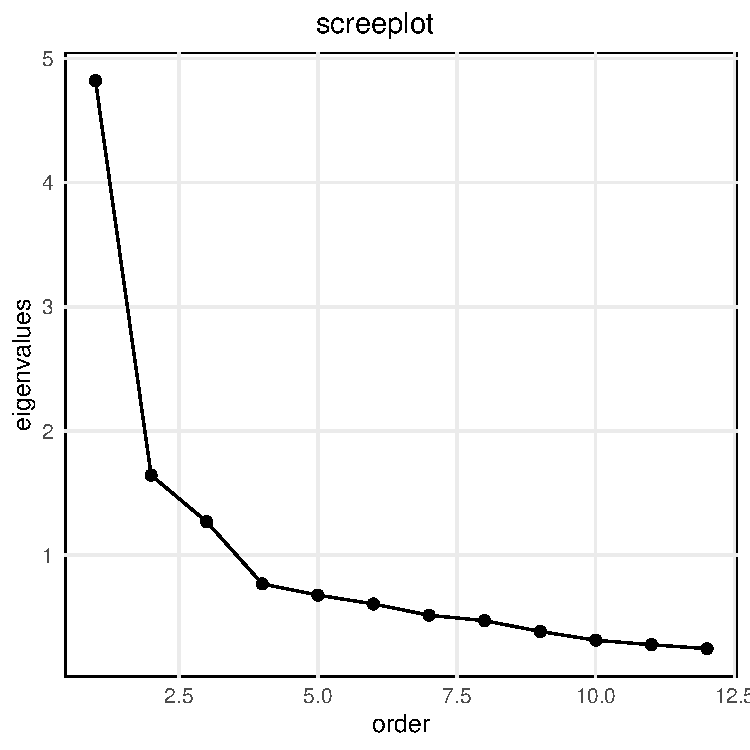
\includegraphics[width = 0.6\textwidth]{spca_JSS-pca_scree.pdf}
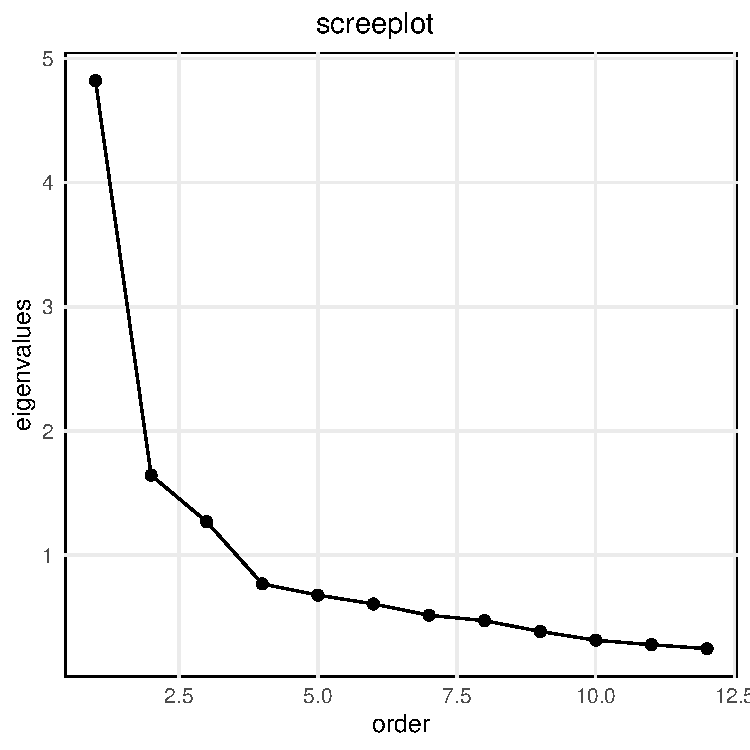
\includegraphics[width = 0.6\textwidth]{spca_JSS-pca_wac.pdf}
\caption{Screeplot.}
\label{fig:screeplot}
\end{figure}
The screeplot in Figure \ref{fig:screeplot} suggests to retain 4 components whereas the qq-plot in Figure \ref{fig:qq-plot} indicates 3. The qq-plot was produced by fitting a line to the first (p - 3) eigenvalues in the plot, setting \code{n_fitline = -3}.
\begin{figure}[H]
\centering
\begin{Schunk}
\begin{Sinput}
R> wachter_qqplot(ho_pca$vexpPC*12, p = ncol(holzinger), 
+                 n = nrow(holzinger), n_fitline = -3)
\end{Sinput}
\end{Schunk}
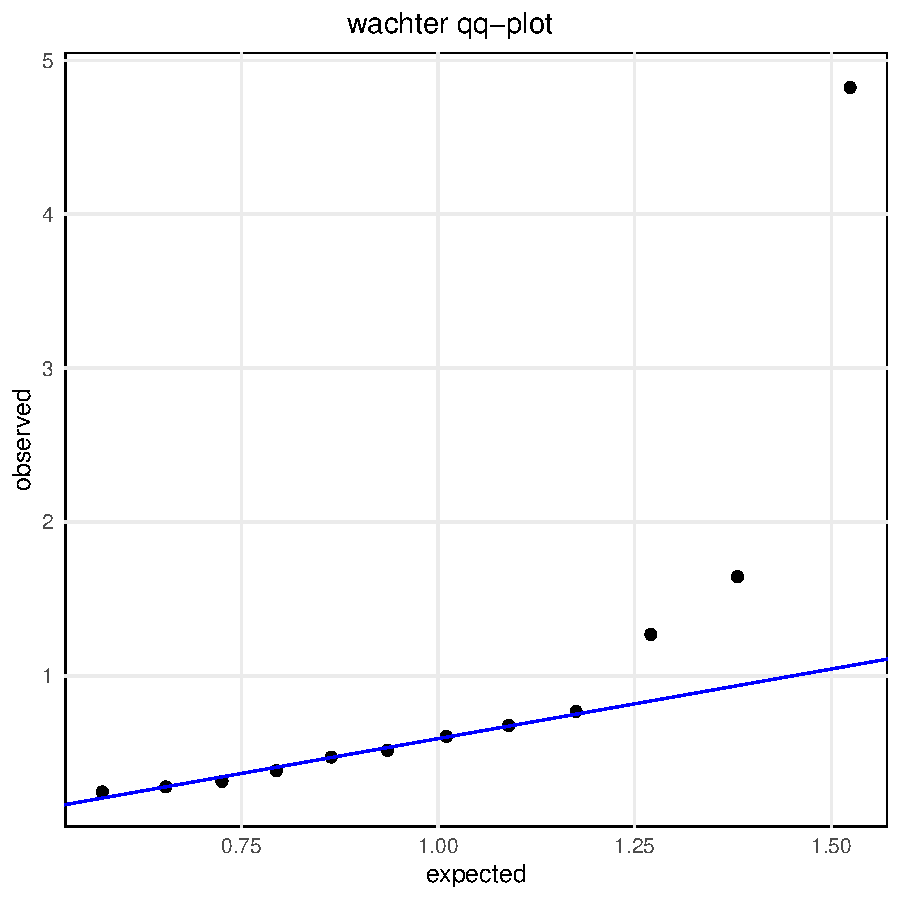
\includegraphics[width = 0.6\textwidth]{spca_JSS-qq-plot.pdf}
\caption{Eigenvalues qq-plot.}
\label{fig:qq-plot}
\end{figure}
We settle for 4 components for caution.  

\subsection{cSPCA fit}
We fit an LSSPCA model with four components,(\code{ncomps = 4}), using the data matrix \code{M} with the default values: \code{alpha = 0.95} is the proportion of objective to reach, CVEXP in this case, note that the function (as all others when a character vector is passed) considers the initial of the first element of the vector in \code{stop_criterion}; \code{method = "c"} indicates that the loadings will be computed with cSPCA; and \code{var_selection = c("fwd", "bkw", "step")} that the variables will be selected with forward selection based on $R^2$, as indicated by \code{intensive = FALSE}.
\begin{Schunk}
\begin{Sinput}
R> ho_spcadef = spca(M = holzinger,
+                    alpha = 0.95,
+                    ncomps = 4,
+                    method = "c",
+                    var_selection = c("fwd", "bkw", "step"),
+                    stop_criterion = c("cvexp", "r2"),
+                    intensive = FALSE
+                    )
\end{Sinput}
\end{Schunk}

The same result could have been produced with \code{ho_spcadef = spca(M = holzinger, ncomps = 4)}.

\subsection{print()}
\fct{print} is the default method and takes the following arguments
\begin{Code}
print.spca = function (x, cols = NULL, only.nonzero = TRUE, 
                contributions = TRUE, digits = 3, thresh = 0.001, 
                return_table = FALSE, components = NULL, ...
                ) 
\end{Code}

By default, percentage contributions are shown (\code{contributions = TRUE}). If \code{only_nonzero = TRUE} (default) the variables that do not load on any sPC are removed.
\begin{Schunk}
\begin{Sinput}
R> ho_spcadef
\end{Sinput}
\begin{Soutput}
            sPC1   sPC2   sPC3   sPC4
visual     11.9%                43.9%
cubes                    31.4% -21.3%
flags      14.2%         23.0%       
paragraph         21.6%              
sentence   19.6%        -29.7%       
wordm             22.3%              
addition   12.2% -27.5% -15.9% -10.6%
counting         -28.6%              
straight   12.3%                     
deduct     13.7%               -24.3%
series     16.1%                     
           -----  -----  -----  -----
Cvexp      38.6%  51.5%  61.4%  67.5%
\end{Soutput}
\end{Schunk}

The argument \code{cols} indicates which columns to print; by default all columns are shown. If an integer is passed, columns \code{1:cols} are shown.  
\subsection{summary()}
Summaries of the \code{spca} output can be produced by calling \code{summary}.
\begin{Schunk}
\begin{Sinput}
R> summary(ho_spcadef)
\end{Sinput}
\begin{Soutput}
        sPC1  sPC2  sPC3  sPC4
Vexp   38.6% 12.9%  9.9%  6.1%
Cvexp  38.6% 51.5% 61.4% 67.5%
Rvexp  96.0% 94.5% 93.5% 95.3%
Rcvexp 96.0% 95.6% 95.3% 95.3%
Card       7     4     4     4
\end{Soutput}
\end{Schunk}

The table shows the following metrics
\begin{itemize}
\item Vexp The percentage variance explained.
\item Cvexp The percentage cumulative variance explained.
\item Rvexp The variance explained relative to the corresponding PC.
\item Rcvexp The cumulative variance explained relative to the 
corresponding PCs.
\item Card  The number of non zero loadings.
\end{itemize}
The cardinality of the sPCs is significantly smaller than the number of features (12) and all sPCs explain more than 95\% of the VEXP of the corresponding PC. The same is true for CVEXP, as required.

Even though the sPCs were computed with cSPCA, so allowing for correlated sPCs, these correlations are quite small (note how sPC4 shows higher correlation).
\begin{Schunk}
\begin{Sinput}
R>  round(ho_spcadef$spc_cor, 2)
\end{Sinput}
\begin{Soutput}
      sPC1 sPC2  sPC3  sPC4
sPC1  1.00 0.01 -0.03 -0.02
sPC2  0.01 1.00  0.08  0.10
sPC3 -0.03 0.08  1.00 -0.06
sPC4 -0.02 0.10 -0.06  1.00
\end{Soutput}
\end{Schunk}

The correlations between sPCs and PCs, shown below, indicates that while the first three sPCs are highly correlated with the corresponding PCs, the fourth is not. Thus confirming that number of important PCs is three, while the fourth is explaining a substancial portion of noise.

\begin{Schunk}
\begin{Sinput}
R>  round(diag(cor(ho_spcadef$scores, ho_pca$scores[, 1:4])), 2)
\end{Sinput}
\begin{Soutput}
[1]  0.98 -0.95  0.92  0.76
\end{Soutput}
\end{Schunk}
sPC4 is negatively correlated with PC4. The sign of the loadings can be easily changed (together with all other internally stored elements) as 
\begin{Schunk}
\begin{Sinput}
R> ho_spcadef = change_loadings_sign_spca(ho_spcadef, 4)
R> round(diag(cor(ho_spcadef$scores, ho_pca$scores[, 1:4])), 2)
\end{Sinput}
\begin{Soutput}
[1]  0.98 -0.95  0.92 -0.76
\end{Soutput}
\end{Schunk}
\subsection{plot()}
The function \code{plot} has several arguments. The arguments grouped in \code{controls} are \pkg{ggplot2} parameters and are included for convenience. The plots can be changed manually after saving the it with \code{return_plot =TRUE}. 
\begin{Code}
plot.spca = function (
 x,
 nplot = NULL,
 plot_type = c("bars", "circular", "heatmap"),
 contributions = TRUE,
 only_nonzero = TRUE,
 pc_loadings = NULL,
 variable_groups = NULL,
 plot_title = NULL,
 return_plot = FALSE,
 produce_plot = TRUE,
 controls = list(
 color_scale = c("ggplot", "cbb", "printsafe", "bw"),
 variable_names = NULL,
 legend_position = c("none", "bottom", "right", "top", "left"),
 grid_type = c("horizontal", "full", "none"),
 facet_labels = NULL,
 legend_title = NULL,
 x_axis_lab = "variables",
 adjust_labels_circ = NULL,
 flip_heatmap = FALSE,
 heatmap_color_range = c("values", "unit")),
 ...) 
\end{Code}
Most arguments' name should be self-explanatory. If a set of PC loadings is passed to \code{PCloadings}, the plots will compare them to the sPCs loadings (not implemented for circular barplots). If a vector or a factor indicating groups of variables is passed to \code{variable_groups}, the plots will show these groups.
\fct{plot} produces three types of plots; the default settings produce a classic barplot, shown in Figure \ref{fig:barplot}

\begin{figure}[H]
\centering
\begin{Schunk}
\begin{Sinput}
R> plot(ho_spcadef)
\end{Sinput}
\end{Schunk}
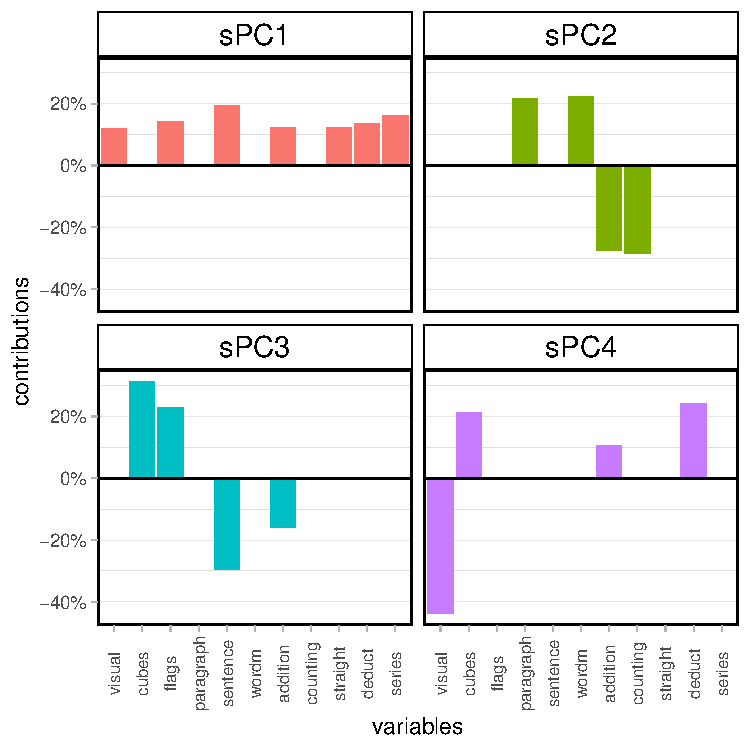
\includegraphics[width = 0.6\textwidth]{spca_JSS-barplot.pdf}
\caption{Bar plots of the contributions of each sPC.}
\label{fig:barplot} 
\end{figure}
A more compact circular plot, shown in Figure \ref{fig:circplot} is produced by selecting \code{plot_type = "c"}
\begin{figure}[H]
\centering
\begin{Schunk}
\begin{Sinput}
R> plot(ho_spcadef, nplot = 3, plot_type = "c")
\end{Sinput}
\end{Schunk}
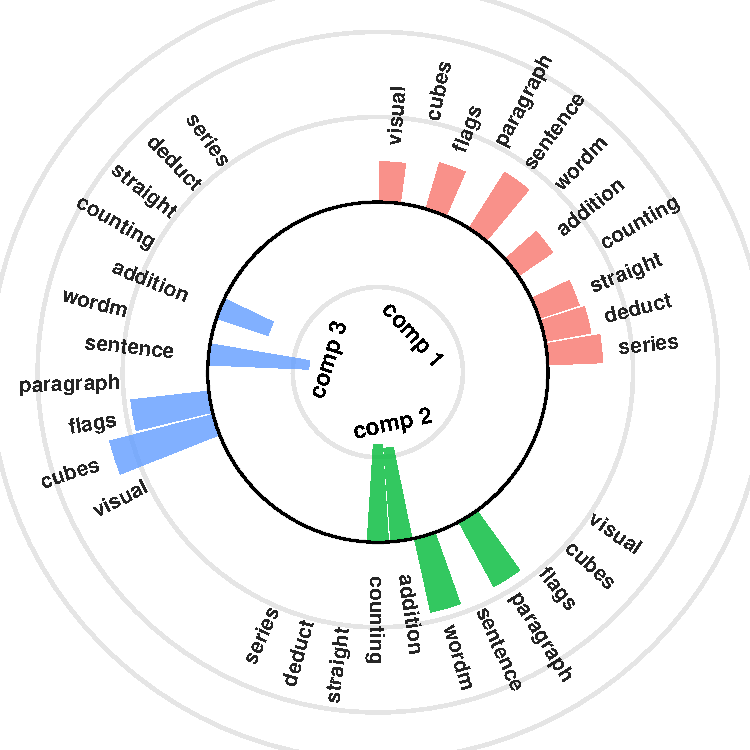
\includegraphics[width = 0.6\textwidth]{spca_JSS-circplot.pdf}
\caption{Circular bar plots of the contributions of each sPC.}
\label{fig:circplot} 
\end{figure}

SPCA contributions can be compared with the PCA contributions with barplots or heat maps, for example using a heat map with both contribution sets depicted.We left the default color range to vary  within the values range (\code{heatmap_color_range = "values"}), rather than between -1 and 1, because in that case colors usually become undistinguishable.

\begin{figure}[H]
\centering
\begin{Schunk}
\begin{Sinput}
R> plot(ho_spcadef, pc_loadings = ho_pca$contributions, plot_type= "h")
\end{Sinput}
\end{Schunk}
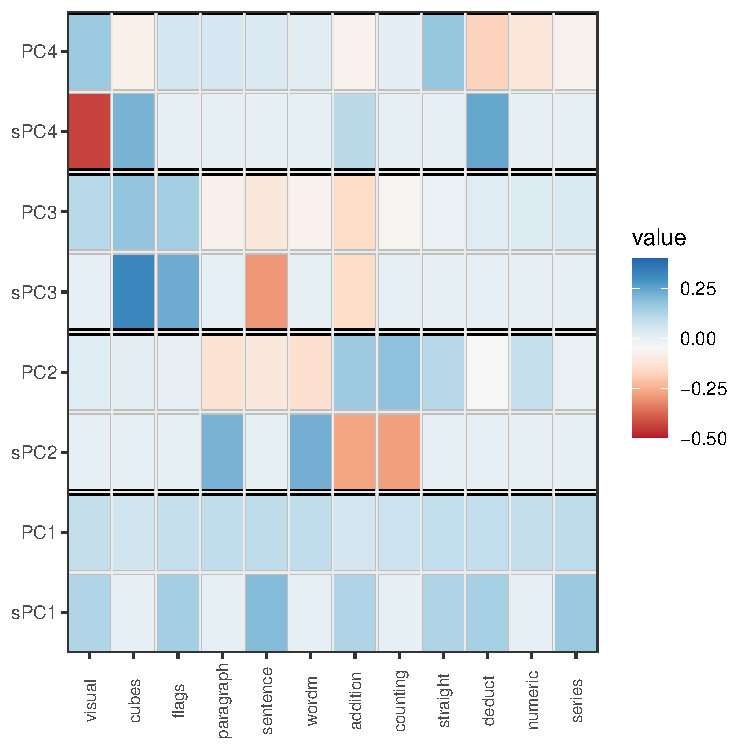
\includegraphics{spca_JSS-heatmap_compare}
\caption{Heatmaps of the contributions of each sPC compared with the corresponding PCs contributions.}
\label{fig:heatmap} 
\end{figure}
\subsection{Other utilities}
\subsubsection{Viewing only nonzero loadings}
Individually nonzero loadings sets are ready avilable in an \code{spca}and contributions can be visualized  by calling \code{show_contributions_spca}
\begin{Schunk}
\begin{Sinput}
R> print("Loadings")
\end{Sinput}
\begin{Soutput}
[1] "Loadings"
\end{Soutput}
\begin{Sinput}
R> ho_spcadef$loadings_list[1:2]
\end{Sinput}
\begin{Soutput}
$sPC1
   visual     flags  sentence  addition  straight    deduct    series 
0.4205005 0.5099249 0.3209397 0.3689273 0.3561735 0.3188142 0.3091023 

$sPC2
 paragraph      wordm   addition   counting 
 0.5672593 -0.4418786  0.5461974 -0.4296842 
\end{Soutput}
\begin{Sinput}
R> show_contributions_spca(ho_spcadef, cols = 1:2)
\end{Sinput}
\begin{Soutput}
$sPC1
   visual     flags  sentence  addition  straight    deduct    series 
0.1614588 0.1957949 0.1232306 0.1416564 0.1367593 0.1224145 0.1186854 

$sPC2
 paragraph      wordm   addition   counting 
 0.2857701 -0.2226067  0.2751597 -0.2164634 

$sPC3
     cubes      flags   sentence   addition 
 0.3135691 -0.2965215  0.2304145 -0.1594949 

$sPC4
    visual      cubes   addition     deduct 
 0.4387985 -0.2131231 -0.2425778 -0.1055006 
\end{Soutput}
\end{Schunk}

\subsubsection{Compare solutions}
We fit a new model requiring that the sPCs have at least 0.95 correlation with the  residual PCs, using pSPCA to compute the loadings and backward elimination to select the variables.

\begin{Schunk}
\begin{Sinput}
R> ho_pspca = spca(holzinger, ncomps = 4, alpha = 0.95,  method = "p",
+                  stop_criterion = "r2", var_selection = "b")
R> round(diag(cor(ho_pspca$scores, ho_pca$scores[, 1:4])), 2)
\end{Sinput}
\begin{Soutput}
[1]  0.98 -0.99  0.98  0.94
\end{Soutput}
\begin{Sinput}
R> ho_psppca = change_loadings_sign_spca(ho_pspca, 4)
\end{Sinput}
\end{Schunk}

Numerical and visual comparisons with \code{ho_spcadef} 
can be obtained calling \code{compare_spca()}. We add methods names to be used in the plot but keep the default argument \code{col_short_names = TRUE} to keep the tables compact.
\begin{Schunk}
\begin{Sinput}
R> ho_compare = compare_spca(list(ho_spcadef, ho_pspca), plot_loadings = TRUE, 
+               print_loadings = TRUE, color_scale = "c", 
+               methods_names = c("cSPCA", "pSPCA")
+               )
\end{Sinput}
\begin{Soutput}
[1] "Percentage Contributions"
          C1.M1 C1.M2 C2.M1 C2.M2 C3.M1 C3.M2 C4.M1 C4.M2
visual     11.9                          12.5 -43.9    20
cubes                              31.4  21.6  21.3      
flags      14.2  11.6                23  17.1            
paragraph        23.7  21.6  15.4       -11.6            
sentence   19.6              13.5 -29.7 -16.2        13.4
wordm                  22.3  16.7                        
addition   12.2       -27.5 -18.8 -15.9 -20.9  10.6      
counting         10.7 -28.6 -20.1                        
straight   12.3  13.9       -15.6                    17.9
deduct     13.7  12.8                          24.3 -22.2
numeric          12.1                               -17.1
series     16.1  15.2                                -9.4
 
[1] Summary statistics
         C1.M1  C1.M2  C2.M1  C2.M2  C3.M1  C3.M2  C4.M1  C4.M2 
Vexp      38.6%  38.6%  12.9%  13.5%   9.9%  10.4%   6.1%   6.4%
Cvexp     38.6%  38.6%  51.5%  52.1%  61.4%  62.5%  67.5%  68.8%
Rvexp     96.0%  96.0%  94.5%  98.5%  93.5%  97.9%  95.3%  99.8%
Rcvexp    96.0%  96.0%  95.6%  96.7%  95.3%  96.9%  95.3%  97.1%
Card          7      7      4      6      4      6      4      6
Min cont  11.9%  10.7%  21.6%  13.5%  15.9%  11.6%  10.6%   9.4%
\end{Soutput}
\begin{Sinput}
R> round(cor(ho_spcadef$scores, ho_pspca$scores), 2)
\end{Sinput}
\begin{Soutput}
     sPC1  sPC2  sPC3  sPC4
sPC1 0.96  0.01 -0.02  0.07
sPC2 0.04  0.96  0.12  0.01
sPC3 0.04 -0.05  0.94 -0.12
sPC4 0.09 -0.01 -0.18 -0.65
\end{Soutput}
\end{Schunk}
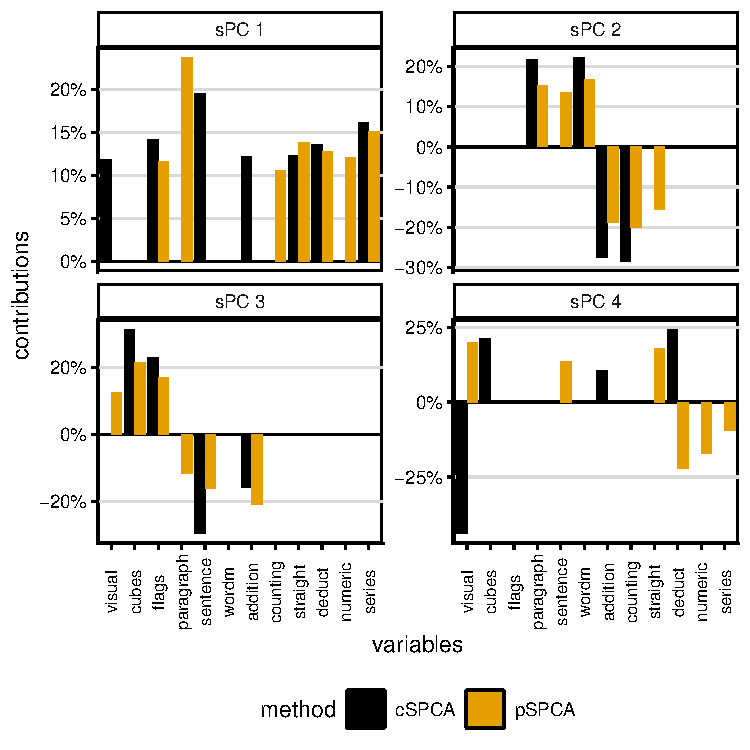
\includegraphics{spca_JSS-compare}

The pSPCA loadings have from the second sPC have larger cardinality and larger VEXP. This is to be expected because VEXP cannot be lower than the $R^2$ optimized. The contributions for the first three sets of loadings are not very dissimilar, considering the the different methods used. The sPCs scores are also are also highly mutually correlated. As noted before, the fourth sPC is unstable.
\subsubsection{Feature groups}
In some cases, typically for questionnaire data, features belong to different groups. For our data the 12 features are grouped in 4 scales. 

The function \code{aggregate_by_group} uses the index vector to sum the loadings or contributions in each scale; adding the vector to \fct{plot} returns plots with scales filled with different colors
\begin{Schunk}
\begin{Sinput}
R> aggregate_by_group(ho_spcadef, groups = holzinger_scales)
\end{Sinput}
\begin{Soutput}
[1] "percentage contributions"
      sPC1   sPC2   sPC3   sPC4
SPL  26.0%   0.0%  54.4% -22.6%
VBL  19.6%  43.9% -29.7%   0.0%
SPD  24.6% -56.1% -15.9%  10.6%
MTH  29.8%   0.0%   0.0%  24.3%
\end{Soutput}
\begin{Sinput}
R> plot(ho_spcadef, variable_groups = holzinger_scales)
\end{Sinput}
\end{Schunk}
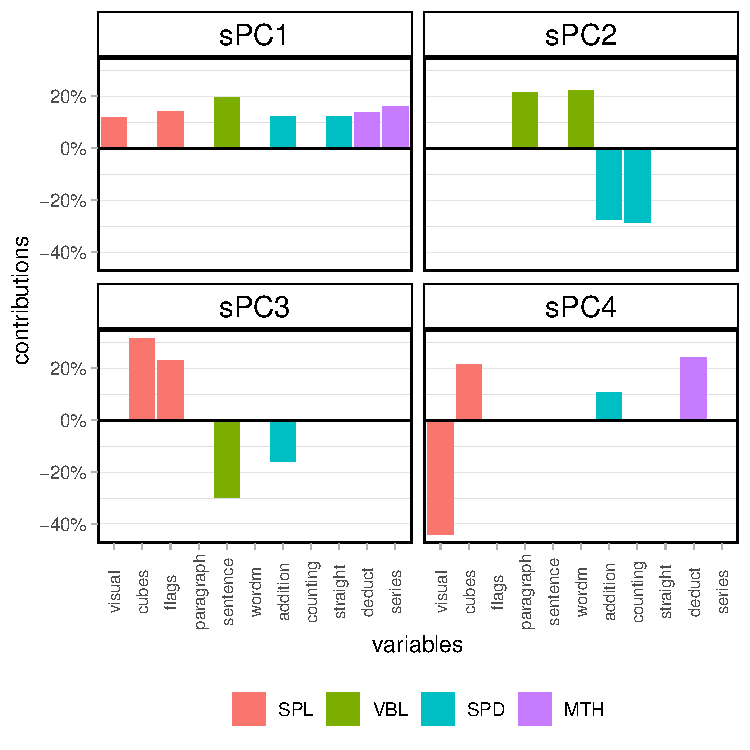
\includegraphics{spca_JSS-aggregate}
\subsubsection{Create an spca object}
\pkg{spca} functions can be applied to results from other analysis by casting them as an \code{spca} object using the \code{new_spca} function. It requires a set of loadings and the covariance (or correlation) matrix needs 
\begin{Schunk}
\begin{Sinput}
R> A = cbind(ho_spcadef$loadings[, 1], ho_pspca$loadings[, 2])
R> ho_r = cor(holzinger)
R> ho_spcahyb = new_spca(A, ho_r, method_name = "hybrid")
R> is.spca(ho_spcahyb)
\end{Sinput}
\begin{Soutput}
[1] TRUE
\end{Soutput}
\begin{Sinput}
R> ho_spcahyb
\end{Sinput}
\begin{Soutput}
            sPC1   sPC2
visual     11.9%       
flags      14.2%       
paragraph         15.4%
sentence   19.6%  13.5%
wordm             16.7%
addition   12.2% -18.8%
counting         -20.1%
straight   12.3% -15.6%
deduct     13.7%       
series     16.1%       
           -----  -----
Cvexp      38.6%  52.1%
\end{Soutput}
\end{Schunk}


\bibliography{JSS}
\end{document}

% \begin{figure}[t!]
% \centering
% <<visualization, echo=FALSE, fig=TRUE, height=5.2, width=7>>=
% par(mar = c(4, 4, 1, 1))
% plot(table(quine$Days), xlab = "Days", ylab = "Frequency", axes = FALSE)
% axis(2)
% axis(1, at = 0:16 * 5, labels = FALSE)
% axis(1, at = 0:8 * 10)
% box()
% @
% \caption{\label{fig:quine} Frequency distribution for number of days absent
% from school.}
% \end{figure}
% 
% \begin{Code}
% glm(formula, data, subset, na.action, weights, offset,
%   family = gaussian, start = NULL, control = glm.control(...),
%   model = TRUE, y = TRUE, x = FALSE, ...)
% \end{Code}
% where \code{formula} plus \code{data}
% 
% <<summary>>=
% summary(m_nbin)
% @
% %%%%%%%%%%%%%%%

